\documentclass[man]{apa6}
\usepackage{lmodern}
\usepackage{amssymb,amsmath}
\usepackage{ifxetex,ifluatex}
\usepackage{fixltx2e} % provides \textsubscript
\ifnum 0\ifxetex 1\fi\ifluatex 1\fi=0 % if pdftex
  \usepackage[T1]{fontenc}
  \usepackage[utf8]{inputenc}
\else % if luatex or xelatex
  \ifxetex
    \usepackage{mathspec}
  \else
    \usepackage{fontspec}
  \fi
  \defaultfontfeatures{Ligatures=TeX,Scale=MatchLowercase}
\fi
% use upquote if available, for straight quotes in verbatim environments
\IfFileExists{upquote.sty}{\usepackage{upquote}}{}
% use microtype if available
\IfFileExists{microtype.sty}{%
\usepackage{microtype}
\UseMicrotypeSet[protrusion]{basicmath} % disable protrusion for tt fonts
}{}
\usepackage{hyperref}
\hypersetup{unicode=true,
            pdftitle={The development of infants' responses to mispronunciations - A Meta-Analysis},
            pdfauthor={Katie Von Holzen~\& Christina Bergmann},
            pdfkeywords={keywords},
            pdfborder={0 0 0},
            breaklinks=true}
\urlstyle{same}  % don't use monospace font for urls
\usepackage{graphicx,grffile}
\makeatletter
\def\maxwidth{\ifdim\Gin@nat@width>\linewidth\linewidth\else\Gin@nat@width\fi}
\def\maxheight{\ifdim\Gin@nat@height>\textheight\textheight\else\Gin@nat@height\fi}
\makeatother
% Scale images if necessary, so that they will not overflow the page
% margins by default, and it is still possible to overwrite the defaults
% using explicit options in \includegraphics[width, height, ...]{}
\setkeys{Gin}{width=\maxwidth,height=\maxheight,keepaspectratio}
\IfFileExists{parskip.sty}{%
\usepackage{parskip}
}{% else
\setlength{\parindent}{0pt}
\setlength{\parskip}{6pt plus 2pt minus 1pt}
}
\setlength{\emergencystretch}{3em}  % prevent overfull lines
\providecommand{\tightlist}{%
  \setlength{\itemsep}{0pt}\setlength{\parskip}{0pt}}
\setcounter{secnumdepth}{0}
% Redefines (sub)paragraphs to behave more like sections
\ifx\paragraph\undefined\else
\let\oldparagraph\paragraph
\renewcommand{\paragraph}[1]{\oldparagraph{#1}\mbox{}}
\fi
\ifx\subparagraph\undefined\else
\let\oldsubparagraph\subparagraph
\renewcommand{\subparagraph}[1]{\oldsubparagraph{#1}\mbox{}}
\fi

%%% Use protect on footnotes to avoid problems with footnotes in titles
\let\rmarkdownfootnote\footnote%
\def\footnote{\protect\rmarkdownfootnote}

%%% Change title format to be more compact
\usepackage{titling}

% Create subtitle command for use in maketitle
\newcommand{\subtitle}[1]{
  \posttitle{
    \begin{center}\large#1\end{center}
    }
}

\setlength{\droptitle}{-2em}
  \title{The development of infants' responses to mispronunciations - A
Meta-Analysis}
  \pretitle{\vspace{\droptitle}\centering\huge}
  \posttitle{\par}
  \author{Katie Von Holzen\textsuperscript{1,2}~\& Christina
Bergmann\textsuperscript{3,4}}
  \preauthor{\centering\large\emph}
  \postauthor{\par}
  \date{}
  \predate{}\postdate{}

\shorttitle{Mispronunciation Meta-Analysis}
\affiliation{
\vspace{0.5cm}
\textsuperscript{1} Language Development Laboratory, University of Maryland, USA\\\textsuperscript{2} Laboratoire Psychologie de la Perception, Université Paris Descartes\\\textsuperscript{3} Max Planck Institute for Psycholinguistics, Nijmegen, the Netherlands\\\textsuperscript{4} LSCP, Departement d'Etudes Cognitives, ENS, EHESS, CNRS, PSL Research University}
\keywords{keywords\newline\indent Word count: X}
\usepackage{csquotes}
\usepackage{upgreek}
\captionsetup{font=singlespacing,justification=justified}

\usepackage{longtable}
\usepackage{lscape}
\usepackage{multirow}
\usepackage{tabularx}
\usepackage[flushleft]{threeparttable}
\usepackage{threeparttablex}

\newenvironment{lltable}{\begin{landscape}\begin{center}\begin{ThreePartTable}}{\end{ThreePartTable}\end{center}\end{landscape}}

\makeatletter
\newcommand\LastLTentrywidth{1em}
\newlength\longtablewidth
\setlength{\longtablewidth}{1in}
\newcommand{\getlongtablewidth}{\begingroup \ifcsname LT@\roman{LT@tables}\endcsname \global\longtablewidth=0pt \renewcommand{\LT@entry}[2]{\global\advance\longtablewidth by ##2\relax\gdef\LastLTentrywidth{##2}}\@nameuse{LT@\roman{LT@tables}} \fi \endgroup}


\DeclareDelayedFloatFlavor{ThreePartTable}{table}
\DeclareDelayedFloatFlavor{lltable}{table}
\DeclareDelayedFloatFlavor*{longtable}{table}
\makeatletter
\renewcommand{\efloat@iwrite}[1]{\immediate\expandafter\protected@write\csname efloat@post#1\endcsname{}}
\makeatother
\usepackage{lineno}

\linenumbers

\authornote{

Correspondence concerning this article should be addressed to Katie Von
Holzen, 0221A LeFrak Hall, University of Maryland, College Park, MD
20742. E-mail:
\href{mailto:katie.m.vonholzen@gmail.com}{\nolinkurl{katie.m.vonholzen@gmail.com}}}

\abstract{
One or two sentences providing a \textbf{basic introduction} to the
field, comprehensible to a scientist in any discipline.

Two to three sentences of \textbf{more detailed background},
comprehensible to scientists in related disciplines.

One sentence clearly stating the \textbf{general problem} being
addressed by this particular study.

One sentence summarizing the main result (with the words ``\textbf{here
we show}'' or their equivalent).

Two or three sentences explaining what the \textbf{main result} reveals
in direct comparison to what was thought to be the case previously, or
how the main result adds to previous knowledge.

One or two sentences to put the results into a more \textbf{general
context}.

Two or three sentences to provide a \textbf{broader perspective},
readily comprehensible to a scientist in any discipline.


}

\usepackage{amsthm}
\newtheorem{theorem}{Theorem}[section]
\newtheorem{lemma}{Lemma}[section]
\theoremstyle{definition}
\newtheorem{definition}{Definition}[section]
\newtheorem{corollary}{Corollary}[section]
\newtheorem{proposition}{Proposition}[section]
\theoremstyle{definition}
\newtheorem{example}{Example}[section]
\theoremstyle{definition}
\newtheorem{exercise}{Exercise}[section]
\theoremstyle{remark}
\newtheorem*{remark}{Remark}
\newtheorem*{solution}{Solution}
\begin{document}
\maketitle

\section{Introduction}\label{introduction}

Acquiring a first language means that young learners are solving a host
of tasks in a short amount of time. As infants develop into toddlers
during their second and third years they learn new words in earnest
while simultaneously refining their knowledge about the sounds that make
up these words. Before children can correctly pronounce a word, they
already show evidence of sensitivity to slight variations in the
phonological form of that word. This mispronunciation sensitivity
reflects the specificity with which infants represent the phonological
information of familiar words and are sensitive to changes that might
signal a change in word meaning. As infants continue to develop into
expert language users, their language processing matures and becomes
more efficient. In a mature phono-lexical system, word recognition must
balance flexibility to slight variation (e.g., speaker identity,
accented speech) while distinguishing between phonetic details that
differentiate words in their native language (e.g.~cat-hat). In this
paper, we aggregate and analyze the almost 20 years of literature
investigating mispronunciation sensitivity in infants in an attempt to
uncover its characteristics and the trajectory of its development.

At the turn of the millenia, infant language acquisition researchers had
established that during their first years of life, infants are sensitive
to changes in the phonetic detail of newly segmented words (Jusczyk \&
Aslin, 1995) and learned minimal pairs (Stager \& Werker, 1997).
Furthermore, when presented with familiar image pairs, children fixate
on one image upon hearing its label (Fernald, Pinto, Swingley, Weinberg,
\& McRoberts, 1998). Swingley and Aslin (2000) were the first to tie
these lines of research together and investigate mispronunciation
sensitivity in infant familiar word recognition: Children aged 18 to 23
months learning American English were presented with pairs of images
(e.g.~baby, dog) and their eye movements to each image were coded
offline. On \enquote{correct} trials, children heard the correct label
for one of the images (e.g.~baby). On \enquote{mispronounced} trials,
children heard a mispronounced label of one of the images (e.g.~vaby).
Mean proportion of fixation to the target image (here: a baby) was
calculated for both correct and mispronounced trials by dividing the
target looking time by the sum of total looking time to both target and
a distractor (proportion of target looking or PTL). Mean fixations in
correct trials were significantly greater than in mispronounced trials,
although looks to the target were significantly greater than chance in
both types of trials. We refer to this pattern of a difference between
looks to correct and mispronounced words as \emph{mispronunciation
sensitivity} and of looks to the target image above chance as
\emph{recognition}. Swingley and Aslin (2000) concluded that already
before the second birthday, children represent words with sufficient
detail to be sensitive to mispronunciations.

The study of Swingley and Aslin (2000) as well as subsequent studies
examining mispronunciation sensitivity address two complementary
concepts in early phonological development: \emph{phonological
constancy} and \emph{phonological distinctiveness}. Phonological
constancy is the ability to accept phonological variation across
different instances of a word, as long as the variation does not
compromise the overall identity of the word. For example, different
speakers - particularly across genders and accents - produce the same
word with notable acoustic variation, although the word remains the
same. In contrast, phonological distinctiveness describes the ability to
differentiate between different words that happen to be phonologically
similar, such as bad/bed or cat/hat. To successfully recognize words,
infants must therefore simultaneously use both phonological constancy
and distinctiveness to determine where phonological variation is
appropriate and where it changes a word's meaning.

In the current study, we focus on infants' developing ability to
correctly apply the principles of phonological distinctiveness and
constancy by using a meta-analytic approach to investigate
mispronunciation sensitivity. Considering that infants are sensitive to
mispronunciations and that, in general, their processing matures with
development, we examine the shape of mispronunciation sensitivity over
the course of the second and third year. There are three distinct
possibilities how mispronunciation sensitivity might change as infants
become native speakers, which are all respectively predicted by
theoretical accounts and supported by single studies. By aggregating all
publicly available evidence using meta-analysis, we can examine
developmental trends making use of data from a much larger and diverse
sample of infants. Before we outline the meta-analytical approach and
its advantages in detail, we first discuss the proposals this study
seeks to disentangle and the data supporting each of the accounts.

Young infants may begin cautiously in their approach to word
recognition, rejecting any phonological variation in familiar words and
only later learning to accept appropriate variability. According to the
Perceptual Attunement account, this describes a shift away from specific
native phonetic patterns to a more mature understanding of the abstract
phonological structure of words (Best 1994, 1995). This shift is
predicted to coincide with the vocabulary spurt around 18 months, and is
therefore related to vocabulary growth. In this case, we would expect
the size of mispronunciation sensitivity to be larger at younger ages
and \emph{decrease} as the child matures and learn more words, although
children continue to detect mispronunciations. Indeed, young infants are
less likely than older infants to demonstrate recognition of familiar
words (Best, Tyler, Gooding, Orlando, \& Quann, 2009; Mulak, Best, \&
Tyler, 2013) or learn new words (Schmale, Hollich, \& Seidl, 2011) from
accented speakers.

According to a different theoretical framework, young infants may
instead begin with phonologically broad representations for familiar
words and only refine their representations as language experience
accumulates. PRIMIR (Processing Rich Information from Multidimensional
Interactive Representations; Curtin \& Werker, 2007; Werker \& Curtin,
2005; Curtin, Byers-Heinlein, \& Werker, 2011) describes the development
of phonemic categories emerging as the number of word form-meaning
linkages increases. Vocabulary growth, therefore, promotes more detailed
phonological representations in familiar words. Following this account,
we predict an \emph{increase} in mispronunciation sensitivity as infants
mature and add more words to their growing lexicon.

Finally, sensitivity to mispronunciation may not be modulated by
development at all. Infants' overall language processing becomes more
efficient, but their sensitivity to mispronunciations may not change.
Across infancy and toddlerhood, mispronunciations would thus be detected
and lead to less looks at a target than correct pronunciations, but the
size of this effect would not change, nor be related to vocabulary size.
This pattern is not predicted by any mainstream theory of language
acquisition, but for completeness we mention it here.

Research following the seminal study by Swingley and Aslin (2000) has
extended mispronunciation sensitivity to infants as young as 12 months
(Mani \& Plunkett, 2010), indicating that from early stages of the
developing lexicon onwards, infants can and do detect mispronunciations.
Regarding the change in mispronunciation sensitivity over development,
however, only a handful of studies have compared more than one age group
on the same mispronunciation task (see Table X), making the current
meta-analysis very informative. One study has found evidence for infants
to become \emph{less} sensitive to mispronunciations as children
develop. Mani and Plunkett (2011) presented 18- and 24-month-olds with
mispronunciations varying in the number of features changed (see below
for a discussion of the role of features). 18-month-olds were sensitive
to mispronunciations, regardless of the number of features changed.
24-month-olds, in contrast, fixated the target image equally for both
correct and 1-feature mispronounced trials, although they were sensitive
to larger mispronunciations. In other words, for 1-feature
mispronunciations at least, sensitivity decreased from 18 to 24 months,
providing support to the prediction that mispronunciation sensitivity
may decrease with development.

In contrast, other studies have found evidence for \emph{greater}
mispronunciation sensitivity as children develop. More precisely, the
difference in target looking for correct and mispronounced trials is
smaller in younger infants and grows as infants develop. Mani and
Plunkett (2007) tested 15-, 18-, and 24-month-olds learning British
English; although all three groups were sensitive to mispronunciations,
15-month-olds showed a less robust sensitivity. An increase in
sensitivity to mispronunciations has also been found from 20 to 24
months (van der Feest \& Fikkert, 2015) and 15 to 18 months (Altvater
Mackensen et al., 2013) in Dutch infants, as well as German infants from
22 to 25 months (Altvater-Mackensen, 2010). Furthermore, van der Feest
and Fikkert (2015) found that sensitivity to specific kinds of
mispronunciations develop at different ages depending on language
infants are learning. In other words, the native language constraints
which \emph{kinds} of mispronunciations infants are sensitive to first,
and that as infants develop, they become sensitive to other
mispronunciations. These studies award support to the prediction that
mispronunciation sensitivity improves with development.

Finally, some studies have found no difference in mispronunciation
sensitivity at different ages. Swingley and Aslin (2000) tested infants
over a wide age range of 5 months (18 to 23 months). They found that age
correlated with target fixations for both correct and mispronounced
labels, whereas the difference between the two (mispronunciation effect)
did not. This suggests that as children develop, they are more likely to
look at the target in the presence of a mispronounced label and that age
is not related to mispronunciation sensitivity. A similar response
pattern has been found for British English learning infants aged between
18 and 24 months (Bailey \& Plunkett, 2002) as well as younger
French-learning infants at 12 and 17 months (Zesiger, Lozeron, Levy, \&
Frauenfelder, 2012). These studies award support to the prediction that
mispronunciation sensitivity does not change with development.

Why would mispronunciation sensitivity change as infants develop, and
would it increase or decrease? The main hypothesis is related to
vocabulary growth. Both the Perceptual Attunement (Best, 1994; 1995) and
PRIMIR (Curtin \& Werker, 2007; Werker \& Curtin, 2005; Curtin,
Byers-Heinlein, \& Werker, 2011) accounts situate a change in
mispronunciation sensitivity occurring along with an increase in
vocabulary size, particularly with the vocabulary spurt at about 18
months. Knowing more words helps infants shift their focus to the
relevant phonetic dimensions needed for word recognition. On the one
hand, a smaller lexicon does not require full specification to
differentiate between words; as more phonologically similar words are
learned, so does the need to have fully detailed representations for
those words (Charles-Luce \& Luce, 1995). On the other hand, a growing
vocabulary is also related to more experience or familiarity with words,
which may sharpen the detail of their representation (Barton, 1980).

Yet, the majority of studies examining a potential association between
mispronunciation sensitivity and vocabulary size have concluded that
there is no relationship (Swingley \& Aslin 2000; 2002; Bailey \&
Plunkett, 2002; Zesiger, Lozeron, Levy, \& Frauenfelder, 2012; Swingley,
2009; Ballem \& Plunkett, 2005; Mani \& Plunkett, 2007; Mani, Coleman,
\& Plunkett, 2008). One notable exception comes from Mani and Plunkett
(2010: keps and tups). Here, 12-month-old infants were divided into a
low vocabulary and high vocabulary group based group median vocabulary
size. High vocabulary infants showed greater sensitivity to vowel
mispronunciations than low vocabulary infants, although this was not the
case for consonant mispronunciations. Taken together, although receiving
considerable support from theories of phono-lexical processing in
language acquisition, there is very little evidence for a role of
vocabulary size in mispronunciation sensitivity. In our current
meta-analysis, we include the relationship between mispronunciation
sensitivity and vocabulary size to further disentangle the disconnect
between theory and experimental results.

Taken together, the studies we have reviewed begin to paint a picture of
the development of mispronunciation sensitivity. Each study contributes
one separate brushstroke and it is only by examining all of them
together that we can achieve a better understanding. Meta-analyses can
not only help us summarize the current state of research, but can also
help us evaluate theories to drive future research and make hands-on
recommendations for experiment planning.

\section{Methods}\label{methods}

The present meta-analysis was conducted with maximal transparency and
reproducibility in mind. To this end, we provide all data and analysis
scripts on the supplementary website (\url{https://osf.io/rvbjs/}) and
open our meta-analysis up for updates (Tsuji, Bergmann, \& Cristia,
2014). The most recent version is available via the website and the
interactive platform MetaLab (metalab.stanford.edu; Bergmann et al.,
2018). Since the present paper was written with embedded analysis
scripts in R {[}@R{]}, it is always possible to re-analyze an updated
dataset. In addition, we follow the Preferred Reporting Items for
Systematic Reviews and Meta-Analyses (PRISMA) guidelines and make the
corresponding information available as supplementary materials (Moher,
Liberati, Tetzlaff, Altman \& PRISMAGroup, 2009). Figure X plots our
PRISMA flowchart.

{[}Figure X. PRISMA Flowchart.{]}
(figures/PRISMA\_MA\_Mispronunciation.png)

\subsection{Study Selection}\label{study-selection}

\begin{tabular}{l|l|l|l}
\hline
Paper & Publication format & Age & Vocabulary\\
\hline
Altvater-Mackensen (2010) & dissertation & 22, 25 & None\\
\hline
Altvater-Mackensen et al. (2014) & paper & 18, 25 & None\\
\hline
Bailey \& Plunkett (2002) & paper & 18, 24 & Comprehension\\
\hline
Bergelson \& Swingley (2017) & paper & 7, 9, 12, 6 & None\\
\hline
Bernier \& White 2017 & proceedings & 21 & None\\
\hline
Delle Luche et al. (2015) & paper & 20, 19 & None\\
\hline
Durrant et al. (2014) & paper & 19, 20 & None\\
\hline
Hoehle et al. 2006 & paper & 18 & None\\
\hline
Hojen et al. & gray paper & 20 & Comprehension/Production\\
\hline
Mani \& Plunkett 2007 & paper & 15, 18, 24, 14, 21 & Comprehension/Production\\
\hline
Mani \& Plunkett 2010 & paper & 12 & Comprehension\\
\hline
Mani \& Plunkett 2011 & paper & 23, 17 & None\\
\hline
Mani, Coleman, \& Plunkett (2008) & paper & 18 & Comprehension/Production\\
\hline
Ramon-Casas \& Bosch 2010 & paper & 24, 25 & None\\
\hline
Ramon-Casas et al. 2009 & paper & 21, 20 & Production\\
\hline
Ren \& Morgan, in press & gray paper & 19 & None\\
\hline
Skoruppa et al. 2013 & paper & 24 & None\\
\hline
Swingley (2009) & paper & 17 & Comprehension/Production\\
\hline
Swingley (2016) & paper & 27, 28 & Production\\
\hline
Swingley \& Aslin (2000) & paper & 20 & Comprehension\\
\hline
Swingley \& Aslin (2002) & paper & 15 & Comprehension/Production\\
\hline
Swingley 2003 & paper & 19 & Comprehension/Production\\
\hline
Tamasi (2016) & dissertation & 30 & None\\
\hline
Tao \& Qinmei 2013 & paper & 12 & None\\
\hline
Tao et al. 2012 & paper & 16 & Comprehension\\
\hline
van der Feest \& Fikkert, 2015 & paper & 24, 20 & None\\
\hline
van der Feest \& Johnson, 2016 & paper & 24 & None\\
\hline
Wewalaarachchi et al. 2017 & paper & 24 & None\\
\hline
White \& Aslin (2011) & paper & 18 & None\\
\hline
White \& Morgan (2008) & paper & 18, 19 & None\\
\hline
Zesiger \& Johr 2011 & paper & 14 & None\\
\hline
Zesiger et al. (2012) & paper & 12, 19 & Comprehension/Production\\
\hline
\end{tabular}

{[}KATIE{]} THIS TABLE IS DEFINITELY NOT FINISHED! {[}CHRISTINA
suggestions: N features should be a range and exclude 0; we could
abbreviate Comperehension/Production to Comp./Prod.,
etcetc{]}{[}KATIE{]} I've reduced the table to be about age and
vocabulary, in order to have it more focused for the aim of this paper.

We first generated a list of potentially relevant items to be included
in our meta-analysis by creating an expert list. This process yielded
110 items. We then used the google scholar search engine to search for
papers citing the original Swingley \& Aslin (2000) publication. This
search was conducted on 22 September, 2017 and yielded 288 results. We
screened the 398 items, removing 99 duplicate items. We screened
remaining 299 items for their title and abstract to determine whether it
met the following inclusion criteria: (1) original data was reported;
(2) the experiment examined familiar word recognition; (3) infants
studied were under 36-months-of-age; (4) the dependent variable was
derived from proportion of looks to a target image versus a distractor
in a eye movement experiment; 5) the stimuli were auditory speech. The
final sample (n = \emph{32}) consisted of 27 journal articles, 1
proceedings paper, 2 thesis, and 2 unpublished reports. We will refer to
these items collectively as papers. Table 1 (Summary Table) provides an
overview of all papers included in the present meta-analysis.

\subsection{Data Entry}\label{data-entry}

The 32 papers we identified as relevant were then coded with as much
detail as possible (Tsuji, Bergmann, \& Cristia, 2014; Bergmann et al.,
2018). For each experiment (note that a paper typically has multiple
experiments), we entered variables describing the publication,
population, experiment design and stimuli, and results. For the present
analyses, we focus on the following characteristics:

1 Condition: Were words mispronounced or not;\\
2 Mean age reported per group of infants, in days;\\
3 Vocabulary size, measured by a standardized questionnaire or list;

We separated out conditions according to whether or not the target word
was mispronounced to be able to investigate infants' looking to the
target picture separated by whether or not words were mispronounced as
well as their mispronunciation sensitivity, which is the difference
between looks to the target in correct and mispronounced trials. When
the same infants were further exposed to multiple mispronunciation
conditions and the results were reported separately in the paper, we
also entered each condition as a separate row (e.g., consonant versus
vowel mispronunciations; Mani \& Plunkett, 2007). The fact that the same
infants contributed data to multiple rows (minimally those containing
information on correct and mispronounced trials) leads to shared
variance across effect sizes, which we account for in our analyses (see
next section). We will call each row a record; in total there were 251
records in our data.

\subsection{Data analysis}\label{data-analysis}

Mispronunciation sensitivity studies typically examine infants'
proportion of target looks (PTL) in comparison to a baseline
measurement. PTL is calculated by dividing the percentage of looks to
the target by the total percentage of looks to both the target and
distractor images. Across papers the baseline comparison varied; we used
the baseline reported by the authors of each paper. Most papers
(\emph{n} = 13) subtracted the PTL score for a pre-naming phase from the
PTL score for a post-naming phase. When interpreting this difference
score, a positive value indicates that infants increased their looks to
the target after hearing the naming label (correct or mispronounced).
Other papers either compared post- and pre-naming PTL with one another
(\emph{n} = 10) or compared post-naming PTL with a chance level of 50\%,
(\emph{n} = 9). For all these comparisons, a positive difference score
or a post-naming phase PTL score that is greater than the pre-naming
phase PTL or chance indicate target looks that indicate object
recognition after hearing the naming label. Consequently, positive
effect sizes reflect more looks to the target picture after naming, and
larger positive effect sizes indicate comparatively more relative
increase in looks to the target.

We report effect sizes for infants' looks to target pictures after
hearing a correctly pronounced or a mispronounced label (object
identification) as well as the difference between effect sizes for
correct and mispronounced trials (i.e.~mispronunciation sensitivity).
The effect size we report in the present paper are based on comparison
of means, standardized by their variance. The most well-known effect
size from this group is Cohen's \emph{d} {[}@cohen{]}. To correct for
the small sample sizes common in infant research, however, we use as a
dependent variable Hedges' \emph{g} instead of Cohen's \emph{d} (Hedges,
1981; Morris, 2000).

We calculated Hedges' \emph{g} using the raw means and standard
deviations reported in the paper (\emph{n} = 2) or using reported
t-values (\emph{n} = 2). Raw means and standard deviations were
extracted from figures for 3 papers. In a within-participation design,
when two means are compared (i.e.~looking during pre- and post-naming)
it is necessary to obtain correlations between the two measurements at
the participant level to calculate effect sizes and effect size variance
based on t-values. Upon request we were provided with correlation values
for one paper (Altvater-Mackensen, 2010); we were able to compute
correlations using means, standard deviations, and t-values for \emph{n}
= 4 (following Csibra, et al. 2016, Appendix B; see also Rabagliati,
Ferguson, \& Lew-Williams, 2018). Correlations were imputed for the
remaining papers (see Black \& Bergmann, 2017, for the same procedure).
We could compute a total of 104 effect sizes for correct pronunciations
and 147 for mispronunciations.

To take into account the fact that the same infants contributed to
multiple datapoints, we analyze our results in a multilevel approach
using the R {[}@R{]} package metafor {[}@metafor{]}. This means we model
as random effect that effect sizes from the same paper share are based
on more similar studies than those across papers and that nested therein
effects can stem from the same infants.

\subsection{Publication Bias}\label{publication-bias}

{[}CHRISTINA: Do you think we have to revise this section? I think it's
the same as in the proceedings paper.{]}{[}KATIE: Are you concerned
about the Publication Bias section in particular, or the Methods as a
whole? In general, some of the Methods was written before the CogSci
paper and in other places to flesh things out I rewrote what we had in
the CogSci paper. Its definitely giving the same information and
sometimes the wording is close, because there's not too many different
ways to explain what a funnel plot is :){]}

In the psychological sciences, there is a documented reluctance to
publish null results. As a result, there is a potential for significant
results to be valued over non-significant results (see Ferguson \&
Heene, 2012). To examine whether this is also the case in the
mispronunciation sensitivity literature, which would bias the data
analyzed in this meta-analysis, we conduct two tests. We first examine
whether effect sizes are distributed as expected based on sampling error
using the rank correlation test of funnel plot asymmetry with the R
{[}@R{]} package metafor {[}@metafor{]}. Effect sizes with low-variance
are expected to fall closer to the estimated mean, while effect sizes
with high-variance should show an increased, evenly-distributed spread
around the estimated mean. Second, we analyze all of the significant
results in the dataset using a p-curve from the p-curve app (v4.0,
p-curve.com; @pcurve). This tests for evidential value by examining
whether the p-values have an expected distribution, regardless of
whether the null hypothesis is true or not, as well as whether there is
a larger proportion of p-values just below the typical alpha threshold
of .05, which may indicate questionable research practices. Responses to
correctly pronounced and mispronounced labels are predicted to show
different patterns of looking behavior; as a result, we conduct these
two analyses to assess publication bias separately for both conditions.

\subsection{Meta-analysis}\label{meta-analysis}

The models reported are hierarchical random-effects models (infant
groups nested within papers) of variance-weighted effect sizes with the
R {[}@R{]} package metafor {[}@metafor{]}. To investigate how
development impacts mispronunciation sensitivity, our core theoretical
question, we introduce age (centered; continuous and measured in days
but transformed into months for ease of reading by dividing by 30.44) as
a moderator to our main model. For the subsequent investigations of
experimental characteristics, we introduce each characteristic as a
moderator (more detail below).

{[}CHRISTINA: Let's both reread the full paper once it is ready and
check that this is properly motivated and whether we do need to list
them all. For now I think the last sentence is fine, but I would tend to
prefer a reminder for the forgetful reader.{]}{[}KATIE: that's
reasonable! We had just listed everything 7 paragraphs before, which
doesn't seem like a lot of \enquote{space}. Alternatively, this
information could be listed in a table, and then just referred to.{]}

\section{Results}\label{results}

\subsection{Publication Bias}\label{publication-bias-1}

Figure 1 shows the funnel plots for both correct pronunciations and
mispronunciations (code adapted from Sakaluk, 2016). Funnel plot
assymmetry was significant for both correct pronunciations (Kendall's
\(\tau\) = 0.53, \emph{p} \textless{} .001) and mispronunciations
(Kendall's \(\tau\) = 0.16, \emph{p} = 0.004). These results,
quantifying the assymmetry in the funnel plots (Figure 1), indicate bias
in the literature. This is particularly evident for correct
pronunciations, where larger effect sizes have greater variance (bottom
right corner) and there are a smaller number of more precise effect
sizes (i.e.~smaller variance) than expected (top left, outside the
triangle).

The stronger publication bias for correct pronunciation might reflect
the status of this condiction as a control. If infants were not looking
to the target picture after hearing the correct label, the overall
experiment design is called into questions. However, due to the small
effect and sample sizes (which we will discuss in the following sections
in more detail) one would expect the regular occurrence of null results
even though as a population infants would reliably show the expected
object identification effect.

We should also point out that funnel plot asymmetry can be caused by
multiple factors beside publication bias. The funnel plot asymmetry may
also reflect heterogeneity in the data, perhaps due to some studies
investigating more subtle effects than other studies. {[}CHRISTINA: I
have to add some bits here.{]}

\subsection{(Insert Figure 1 about
here)}\label{insert-figure-1-about-here}

\begin{verbatim}
## pdf 
##   2
\end{verbatim}

\begin{figure}[htbp]
\centering
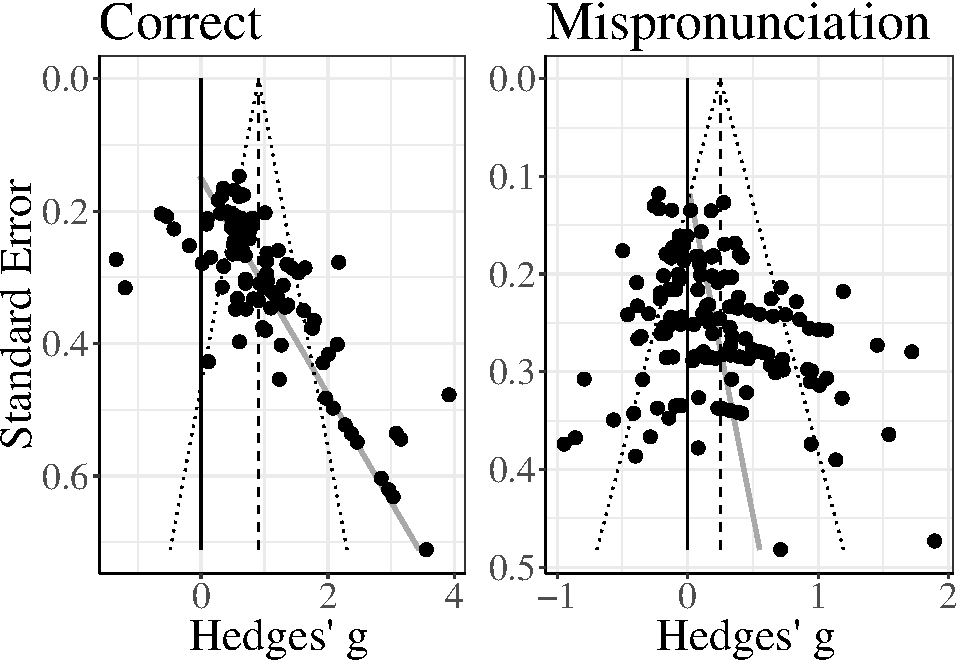
\includegraphics{Paper_Analyses_files/figure-latex/FunnelCombo-1.pdf}
\caption{}
\end{figure}

\begin{verbatim}
## [1] TRUE
\end{verbatim}

\begin{verbatim}
## [1] TRUE
\end{verbatim}

We next examined the p-curves for significant values from the correctly
pronounced and mispronounced conditions. The p-curve based on 72
statistically significant values for correct pronunciations indicates
that the data contain evidential value (Z = -17.93, \emph{p} \textless{}
.001) and there is no evidence of a large proportion of p-values just
below the typical alpha threshold of .05. The p-curve based on 36
statistically significant values for mispronunciations indicates that
the data contain evidential value (Z = -6.81, \emph{p} \textless{} .001)
and there is no evidence of a large proportion of p-values just below
the typical alpha threshold of .05.

Taken together, the results suggest a tendency in the literature towards
publication bias. As a result, our meta-analysis may systematically
overestimate effect sizes and we therefore interpret all estimates with
caution. Yet, the p-curve analysis suggests that overall, the literature
contains evidential value, reflecting a \enquote{real} effect. We
therefore continue our meta-analysis.

\subsection{Meta-analysis}\label{meta-analysis-1}

\subsubsection{Object Identification for Correct and Mispronounced
Words}\label{object-identification-for-correct-and-mispronounced-words}

We first calculated the meta-analytic effect for object identification,
i.e.~looks to the target image in response to correctly pronounced
words. The variance-weighted meta-analytic effect size Hedges' \emph{g}
was 0.908 (SE = 0.12) which was significantly different from zero (95\%
CI{[}0.673, 1.143{]}, \emph{p} \textless{} .001). This is a rather large
effect size (according to the criteria set by Cohen, 1988; see also
Bergmann, et al., 2018; for comparative meta-analytic effect sizes in
language acquisition research). That the effect size is significantly
above zero suggests that when presented with the correctly pronounced
label, infants fixated the corresponding object. Our analysis of funnel
plot asymmetry, however, found evidence for publication bias, which
might lead to an overestimated effect sizes as smaller, non-significant
results might not be published. Although the effect size Hedges'
\emph{g} may be overestimated for object identification in response to
correctly pronounced words, the p-curve results and a CI lower bound of
0.67 suggests that this result is robust even when correcting for
publication bias. In other words, we are confident that the true
population mean lies above zero for object recognition of correctly
pronounced words.

{[}CHRISTINA: Can you explain what the CI lower bound means here? I
don't follow.{]}{[}KATIE: What do you think about this (last sentence)?
The CI lower bound stuff here actually comes from something you wrote,
so tell me whether its correct.{]}

We then calculated the meta-analytic effect for object identification in
response to mispronounced words. In this case, the variance-weighted
meta-analytic effect size Hedges' \emph{g} was 0.25 (SE = 0.06) which
was also significantly different from zero (95\% CI{[}0.133, 0.367{]},
\emph{p} \textless{} .001). This is considered a small effect size
(Cohen, 1988), but significantly above zero, which suggests that even
when presented with a mispronounced label, infants fixated the correct
object. In other words, infants are able to resolve mispronunciations, a
key skill in language processing We again note the publication bias
(which was smaller in this condition), and the possibility that the
effect size Hedges' \emph{g} may be overestimated. But, as the p-curve
indicated evidential value, we are confident in the overall patterns,
namely that infants fixate the target even after hearing a mispronounced
label.

Heterogeneity was significant for both correctly pronounced (Q(103) =
625.63, \emph{p} \textless{} .001) and mispronounced words, (Q(146) =
462.51, \emph{p} \textless{} .001). This indicated that the sample
contains unexplained variance leading to significant difference across
our studies beyond what is to be expected based on random sampling
error. We therefore continue with our moderator analysis.

\subsubsection{Mispronunciation Sensitivity Meta-analytic
Effect}\label{mispronunciation-sensitivity-meta-analytic-effect}

The above two analyses considered the data from mispronounced and
correctly pronounced words separately. To evaluate mispronunciation
sensitivity, we compared the effect size Hedges' \emph{g} for correct
pronunciations with mispronunciations directly, merging the two
datasets. The moderator test was significant, QM(1) = 215.761,
\emph{p}\textless{} .001. Hedges' \emph{g} for mispronunciation
sensitivity was 0.495 (SE = 0.034), which indicated that the responses
across conditions were significantly different (95\% CI{[}0.429,
0.561{]}, \emph{p} \textless{} .001). This confirms that although
infants fixate the correct object for both correct pronunciations and
mispronunciations, the observed fixations to target (as measured by the
effect sizes) were significantly greater for correct pronunciations. In
other words, we observe a significant difference between the two
conditions and can now quantify the modulation of fixation behavior in
terms of standardized effect sizes.

\subsubsection{Object Recognition and Mispronunciation Sensitivity
Modulated by
Age}\label{object-recognition-and-mispronunciation-sensitivity-modulated-by-age}

To evaluate the different predictions we laid out in the introduction
for how mispronunciation sensitivity will change as infants develop, we
next added the moderator age (centered, in days). In the first analyses,
we investigate the impact of age separately on conditions where words
were either pronounced correctly or not. Age did not significantly
modulate object identification in response to correctly pronounced QM(1)
= 215.761, \emph{p}\textless{} .001 or mispronounce words QM(1) =
215.761, \emph{p}\textless{} .001. The lack of a significant modulation
together with the small estimates indicates that there was no
relationship between age and target looks in response to a correctly
pronounced or mispronounced label. This relationship is plotted in
Figure 2.

We then examined the interaction between age and mispronunciation
sensitivity (correct vs.~mispronounced words) in our whole dataset. The
moderator test was significant QM(1) = 215.761, \emph{p}\textless{}
.001. This result is in line with the general observation that as
infants mature they become better at language processing. The
interaction between age and mispronunciation sensitivity, however, was
not significant \(\beta\) = 0.003, SE = 0.008, 95\% CI{[}-0.012,
0.018{]}, \emph{p}= 0.731. The small estimate size, as well as
inspection of Figure 2 suggests that as infants age, their
mispronunciation sensitivity remains the same.

\subsection{(Insert Figure 2 about
here)}\label{insert-figure-2-about-here}

\begin{verbatim}
## pdf 
##   2
\end{verbatim}

\begin{figure}[htbp]
\centering
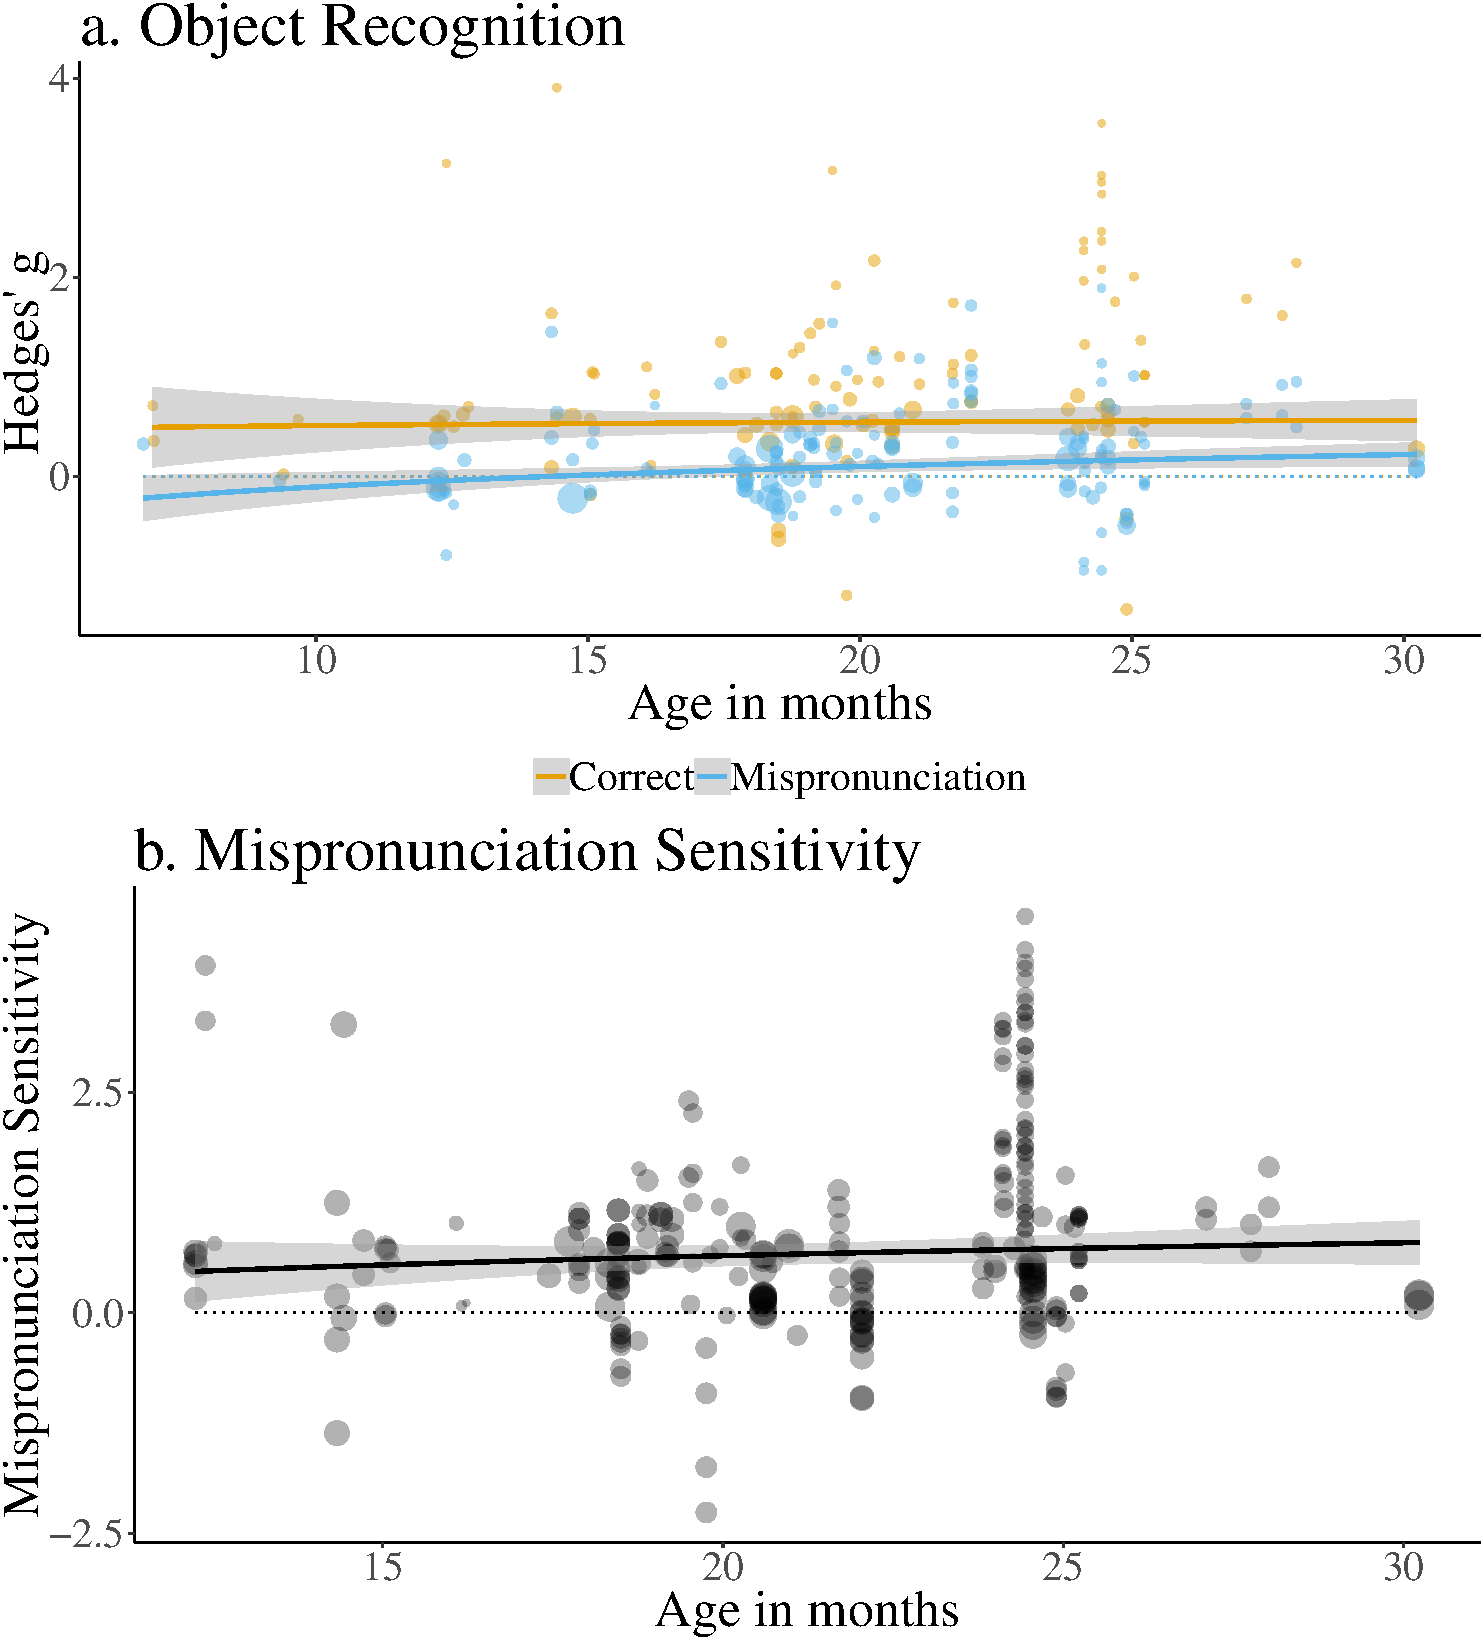
\includegraphics{Paper_Analyses_files/figure-latex/PlotMPEffect-1.pdf}
\caption{}
\end{figure}

\subsubsection{Vocabulary Size: Correlation Between Mispronunciation
Sensitivity and
Vocabulary}\label{vocabulary-size-correlation-between-mispronunciation-sensitivity-and-vocabulary}

Of the 32 papers included in the meta-analysis, 8 (comprehension = 7
papers; production = 1) analyzed the relationship between vocabulary
scores and mispronunciation sensitivity, specifically object recognition
for correct pronunciations and mispronunciations. There is reason to
believe that production data are different from comprehension data (the
former being easier to estimate for parents in the typical
questionnaire-based assessment), so we analyze this data separately.

{[}CHRISTINA{]} SO WE DON'T WANT TO INTERPRET THE FIXED EFFECTS MODEL AT
ALL, IT IS NOT SUITABLE BECAUSE THERE IS VARIANCE BETWEEN EVERY RECORD
(LANGUAGE ETC). I WOULD INTERPRET THE OVERALL CORRELATION AND THE CI,
NOT THE P-VALUE (IN GENERAL). I ALSO WONDER WHETHER WE SHOULD MOVE THE
SUBSET ANALYSES TO THE SUPPLEMENTARY MATERIALS AND JUST SAY OVERALL WE
SEE NO RELATIONSHIPS AND CORRELATION COEFFICIENTS CONSISTENYL BELOW .1
WE THEREFORE MUST CONCLUDE THAT WITHIN NARROW AGE GROUPS VOCABULARY DOES
NOT INFLUENCE ANYTHING WE LOOK AT. WE CANNOT DO THIS ANALYSIS FPOR MP
SENSITIVITY BECAUSE WE DON'T HAVE THE NECESSARY RAW DATA. {[}KATIE: Ah,
so because for each paper the correlation and CI values straddle 0, this
indicates that there really isn't much evidence for a relationship? I've
tried to write this out below, let me know what you think. Over the
summer, I had also played around with looking at how collection of
vocabulary data has dropped off over the years, even though more
mispronunciation studies have been published. That might be something
interesting to add. If we truly think that this is what is driving the
development of mispronunciation sensitivity, then why are people not
collecting this data?{]} (BUT I WONDER WHETHER WECOULD ENCODE THE
REPORTED INTERACTION TERMS AND THE CORRELATION AND THEN DO SOMETHING
WITH THAT?) {[}KATIE: I'm not really sure what you mean by this :({]}

{[}Katie: below, I'm using coweeta.uga.edu/publications/10436.pdf, page
80 as a model for writing up these results. I haven't the funniest clue
what I'm doing! :p{]}

We first considered the relationship between vocabulary and object
recognition for correct pronunciations. Higher comprehension scores were
associated with greater object recognition in response to correct
pronunciations for 9 of 12 experimental conditions, with correlation
values ranging from -0.17 to 0.48. The mean effect size XXX was 0.0897,
but did not differ significantly from zero (95\% CI{[}-0.0105; 0.1900{]}
\emph{p} = .0795). Higher production scores were also associated with
greater object recognition in response to correct pronunciations for 9
of 16 experimental conditions, with correlation values ranging from
-0.23 to 0.44. The mean effect size XXX was 0.0601, but did not differ
significantly from zero (95\% CI{[}-0.0331; 0.1533{]} \emph{p} = .2061).
For both comprehension and production scores, the small correlation
effect sizes and large variances suggest a lack of relationship between
vocabulary and object recognition for correct pronunciations.

We next considered the relationship between vocabulary and object
recognition for mispronunciations. Higher comprehension scores were
associated with greater object recognition in response to correct
pronunciations for 17 of 31 experimental conditions, with correlation
values ranging from -0.35 to 0.57. The mean effect size XXX was 0.0377,
but did not differ significantly from zero (95\% CI{[}-0.0260; 0.1014{]}
\emph{p} = .2465). For production, however, lower production scores were
associated with greater object recognition in response to
mispronunciations for 16 of 31 experimental conditions, with correlation
values ranging from -0.28 to 0.44. The mean effect size XXX was -0.0402,
but did not differ significantly from zero (95\% CI{[}-0.1043; 0.0238{]}
\emph{p} = .2181). For both comprehension and production scores, the
small correlation effect sizes and large variances suggest a lack of
relationship between vocabulary and object recognition for
mispronunciations.

\subsubsection{Interim Discussion}\label{interim-discussion}

The main goal of this paper was to assess mispronunciation sensitivity
and its maturation with age. The results are clear: Although infants
consider a mispronunciation as a better match with the target image than
a distractor image, there was a consistent effect of mispronunciation
sensitivity. This did not change with development. Of the 3 predictions
and assumptions about the development of infants' sensitivity to
mispronunciations discussed in the Introduction, the present results
lend some support for the argument that mispronunciation sensitivity
stays consistent as infants develop. This runs counter to existing
theories of phono-lexical development, which predict either an increase
(PRIMR ref) or decrease (Assim Model ref) in mispronunciation
sensitivity. Furthermore, counter to the predictions for the PRIMR
(PRIMR ref) and Assimilation(Assim ref) models, we found no relationship
between vocabulary and target looking for correct pronunciations or
mispronunciations. In sum, it seems that current theories of infants'
phono-lexical development cannot fully capture our results and should be
reconsidered with all the evidence in mind.

Alternatively, it is possible that variation in the analysis approach
lead to systematic differences in the size of mispronunciation
sensitivity. Choices about the approach to data analysis have a higher
possibility to be influenced by the shape of the data itself after
collection, and are therefore susceptible to a higher rate of
false-positives (Simmons, Nelson, \& Simonsohn, 2011). Although we did
not have specific predictions about these variables, such as size of
time window analyzed or dependent variable calculated, we included these
variables in our coding scheme for the meta-analysis dataset. As
reported in the Methods section (and discussed in detail below), some of
these variables varied widely across studies. In the following section,
we include an exploratory analysis to investigate the possibility of
systematic differences in the approach to analysis in general and across
infant age.

{[}KATIE{]} I've changed the above paragraph to lead to exploratory
analyses, not moderators. Since the fmailiar/unfamiliar analysis doesn't
really work out except for if we kind of subset and torture the data, I
think its more interesting to talk about how choices of analysis /
researcher degrees of freedom may influence the data

\subsection{Exploratory Analyses}\label{exploratory-analyses}

We identified several variables to assess the influence of data analysis
choices. These variables fall into two types of categories: time-related
and dependent variable related. In the following analyses, we discuss
the theoretical motivation for these data analysis choices, the
variation present in the current meta-analysis dataset, and the
influence these choices have on mispronunciation sensitivity
development.

\subsubsection{Time-related analyses}\label{time-related-analyses}

When designing mispronunciation sensitivity studies, experimenters
choose the length of time each trial is presented. This includes both
the length of time before the target object is named (pre-naming phase)
as well as after (post-naming phase) and is determined prior to data
collection. Across papers, trial length varied from 2750 to 13000 ms,
with a mode of 5000 ms. There was an inverse relationship between infant
age and trial length, such that younger infants were given trials of a
longer length, although this correlation was not significant (\emph{r} =
-0.11, \emph{p} = 0.086). Presumably, younger infants may be given
longer trials because their word recognition abilities may be slower
than older infants (Fernald et al., 1998).

Unlike the length of trial, the length of the post-naming phase analyzed
can be chosen after the experimental data is collected. Interestingly,
half of the experimental conditions were analyzed using the same length
of post-naming phase as the infant heard in the actual experiment 126,
while the other half were analyzed using a shorter length of post-naming
phase, excluding later portions of the post-naming phase 125. Across
papers, the length of the post-naming phase analyzed varied from 1510 to
6000 ms, with a mode of 2000 ms. Similar to trial length, there was an
inverse relationship between infant age and length of post-naming phase
analyzed, such that younger infants were analyzed using a longer length
of post-naming phase, although here the relationship was significant
(\emph{r} = -0.21, \emph{p} \textless{} .001). Again, the choice to
analyze a shorter post-naming time window is likely related to evidence
that speed of processing is slower in younger infants (Fernald et al.,
1998). Furthermore, the proportion of post-naming phase time window
analyzed in comprison to the total post-naming phase presented to
infants significantly decreased with increasing infant age (\emph{r} =
-0.18, \emph{p} = 0.004). Although trial length did not differ by infant
age, the size of the post-naming phase time window analyzed did differ
by infant age.

When analyzing eye-movements, it is important to consider the amount of
time it takes for an eye movement to be initiated in response to a
stimulus. Previous studies examining simple stimulus response latencies
first determined that infants require at least 233 ms to initiate an
eye-movement in response to a stimulus (Canfield \& Haith, 1991). In
mispronunciation sensitivity studies, however, this has often been
extended to 367 ms (e.g.~Swingley \& Aslin, 2000, 2002, 2007). Across
papers, the majority used a similar offset value (between 360 and 370
ms) for analysis (\emph{n} = 151), but offset values ranged from 0 to
500 ms, and were not reported for 36 experimental conditions. We note
that Swingley (2009) also included offset values of 1133 ms to analyze
responses to coda mispronunciations. There was an inverse relationship
between infant age and size of offset, such that younger infants were
given longer offsets, although this correlation was not significant
(\emph{r} = -0.10, \emph{p} = 0.13). This lack of a relationship is
perhaps driven by the field's consensus that an offset of about 367 ms
is appropriate for analyzing word recognition with PTL measures,
including studies that evaluate mispronunciation sensitivity.

Although there are a priori reasons to choose the post-naming time
window (infant age) or offset time (previous studies), these choices may
occur after data collection and are therefore susceptible to a higher
rate of false-positives. Considering that differences in these choice
were systematically different across infant ages, at least for the
post-naming time window, we next explored whether the size of the
analyzed post-naming phase time window or the offset time influenced
sensitivity to mispronunciations.

\subsubsection{Length of post time}\label{length-of-post-time}

We first assessed whether size of post-naming phase analyzed had an
impact on the size of mispronunciation sensitivity. First, we calculated
the meta-analytic effect for object identification in response to
mispronounced target words/images, including post-naming phase size as a
moderator. The moderator test was not significant QM(1) = 215.761,
\emph{p}\textless{} .001 and the estimate for post-naming phase size was
relatively small, \(\beta\) = 0.121, SE = 0.073, 95\% CI{[}-0.022,
0.264{]}, \emph{p}= 0.097. This suggests that upon hearing a
mispronunciation, infants' looks to the target image were similar
regardless of the size of the post-naming phase analyzed. We next
assessed whether post-naming phase size was related to mispronunciation
sensitivity. We merged the two datasets and included condition (correct
pronunciation, mispronunciation) as an additional moderator. The
moderator test was significant, QM(1) = 215.761, \emph{p}\textless{}
.001. The estimate for the interaction between post-naming phase size
and condition was small but significant \(\beta\) = -0.156, SE = 0.051,
95\% CI{[}-0.256, -0.056{]}, \emph{p}= 0.002. This relationship is
plotted in Figure 3a. The results suggest that although the size of the
post-naming phase analyzed did not impact infants' likelihood to fixate
the target upon hearing the mispronunciation, it did significantly
impact mispronunciation sensitivity. Specifically, the difference
between target fixations for correctly pronounced and mispronounced
items (mispronunciation sensitivity) was significantly greater when the
post-naming phase that was shorter in length.

Considering that we also found a relationship between the length of the
post-naming phase analyzed and infant age, such that younger ages had a
longer post-naming phase time window of analysis, we next examined
whether the size of post-naming phase analyzed modulated the development
of mispronunciation sensitivity. For object recognition in response to a
mispronunciation, including age as a moderator resulted in a moderator
test that was not significant QM(1) = 215.761, \emph{p}\textless{} .001,
and a small estimate for the interaction between age and size of
post-naming phase (\(\beta\) = -0.156, SE = 0.051, 95\% CI{[}-0.256,
-0.056{]}, \emph{p}= 0.002. This suggests that upon hearing a
mispronunciation, infant measured looks to the target image were
similar, regardless of infant age or size of the post-naming phase
analyzed. We next assessed whether the relationship between size of the
post-naming phase analyzed and mispronunciation sensitivity was
modulated by age. We merged the two datasets and included condition
(correct pronunciation, mispronunciation) as well as age as additional
moderators. The moderator test was significant QM(1) = 215.761,
\emph{p}\textless{} .001. The estimate for the three-way-interaction
between condition, size of post-naming phase, and age was small, but
significant (\(\beta\) = = NA, SE = NA, 95\% CI{[}NA, NA{]}, \emph{p}NA.
This relationship is plotted in Figure 3b. Smaller post-naming phase
size lead to greater increases in mispronunciation sensitivity with
development. For example, experimental conditions analyzed with a
post-naming phase of 2000 ms or less, mispronunciation sensitivity
increases with infant age, whereas a post-naming phase of greater than
2000 ms leads to either no impact of age on mispronunciation sensitivity
or a negative relationship between age and mispronunciation sensitivity.

\subsection{(Insert Figure 3 about
here)}\label{insert-figure-3-about-here}

\begin{verbatim}
## pdf 
##   2
\end{verbatim}

\begin{figure}[htbp]
\centering
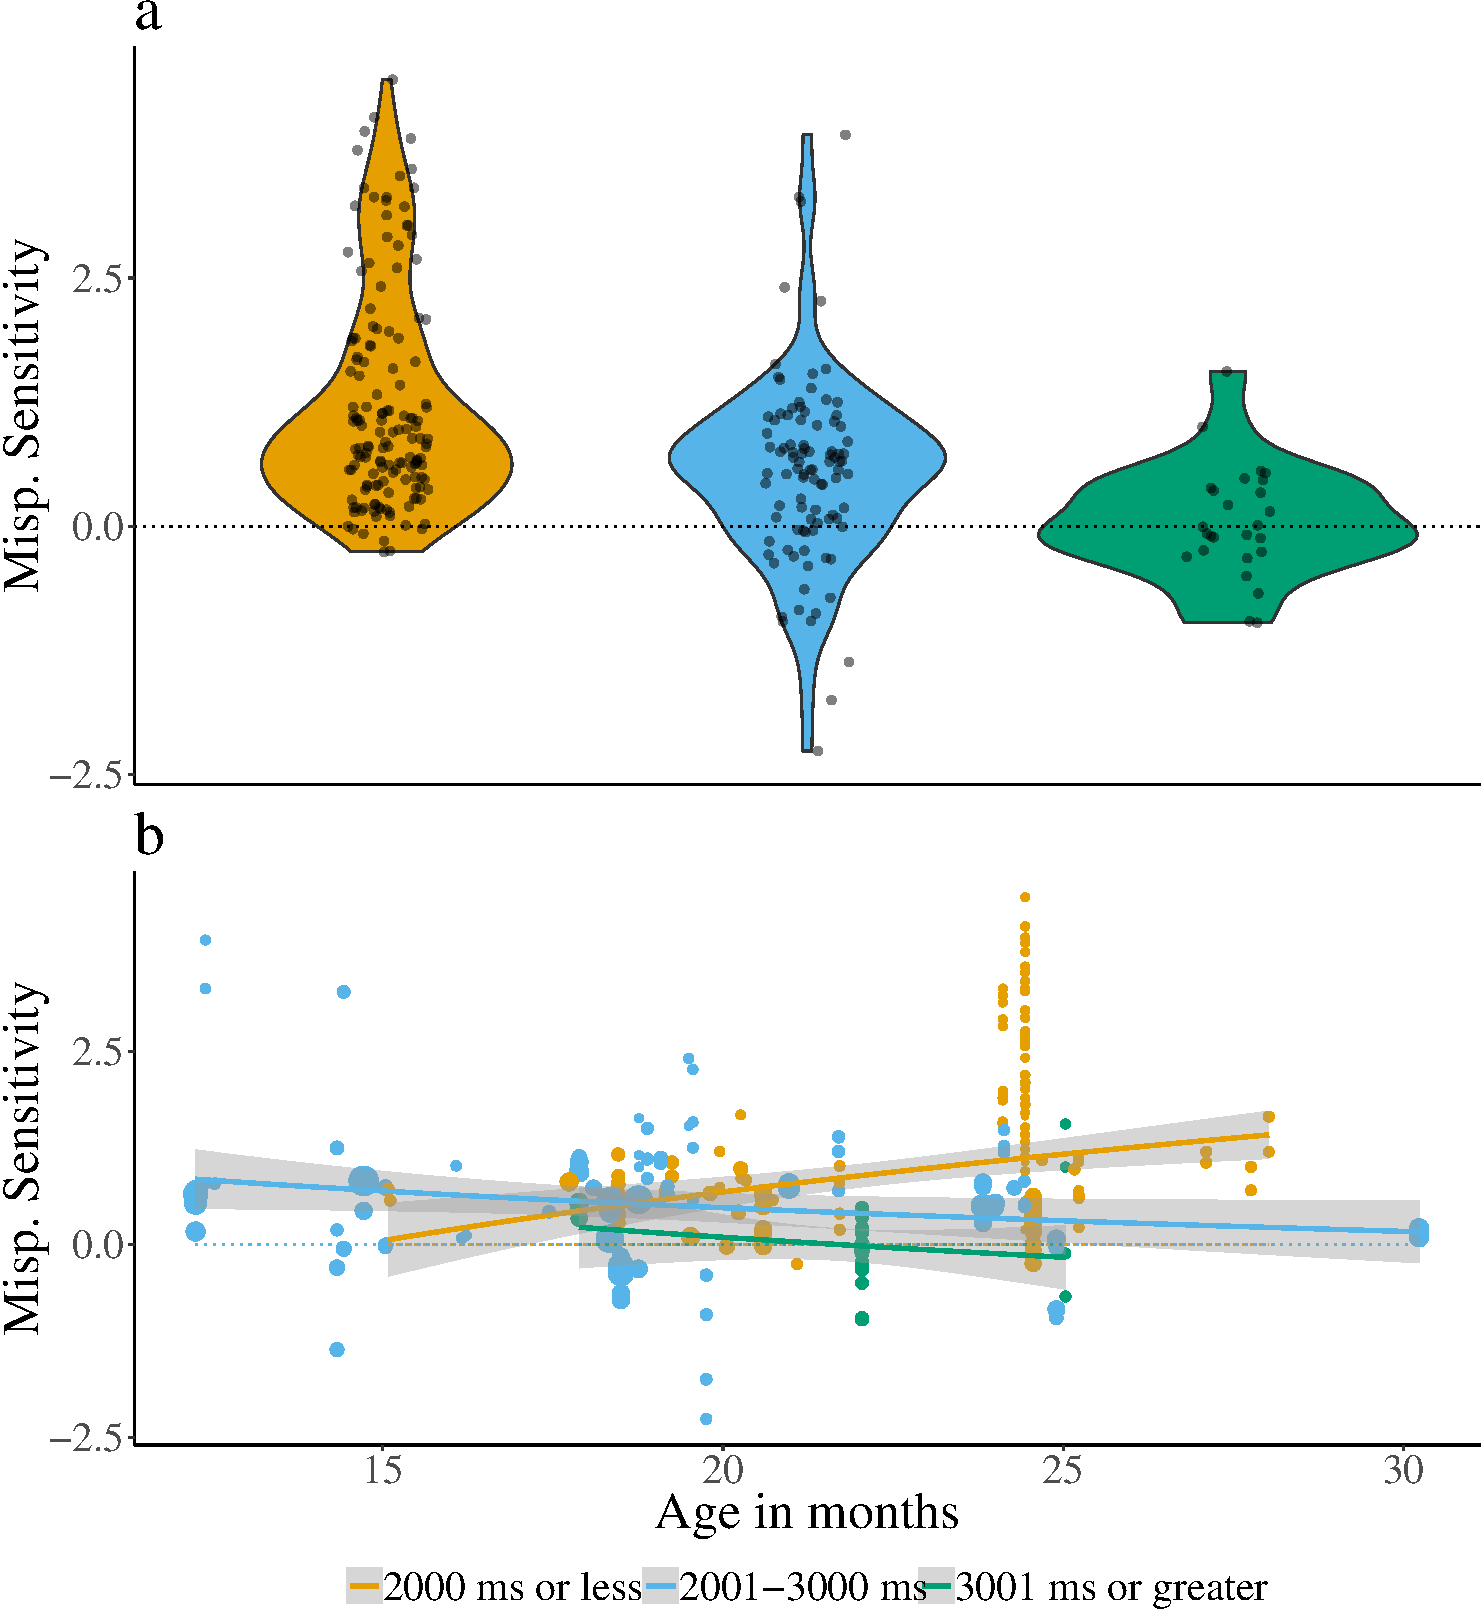
\includegraphics{Paper_Analyses_files/figure-latex/Plot_post_name_cond_age-1.pdf}
\caption{}
\end{figure}

\subsubsection{Length of offset time}\label{length-of-offset-time}

We next assessed whether offset time had an impact on the size of
mispronunciation sensitivity. First, we calculated the meta-analytic
effect for object identification in response to mispronounced target
words/images, including offset time as a moderator. The moderator test
was not significant QM(1) = 215.761, \emph{p}\textless{} .001 and the
estimate for offset time was very small, \(\beta\) = 0.001, SE = 0, 95\%
CI{[}0, 0.001{]}, \emph{p}= 0.132. This suggests that upon hearing a
mispronunciation, infants' looks to the target image were similar
regardless of the offset time used to analyze the data. We next assessed
whether offset time was related to mispronunciation sensitivity. We
merged the two datasets and included condition (correct pronunciation,
mispronunciation) as an additional moderator. The moderator test was
significant, QM(1) = 215.761, \emph{p}\textless{} .001, but the estimate
for the interaction between offset time and condition was very small and
not significant \(\beta\) = 0, SE = 0, 95\% CI{[}-0.001, 0{]}, \emph{p}=
0.505.

We next examined whether offset time modulated the development of
mispronunciation sensitivity. For object recognition in response to a
mispronunciation, including age as a moderator resulted in a moderator
test that was not significant QM(1) = 215.761, \emph{p}\textless{} .001,
and a very small estimate for the interaction between age and size of
post-naming phase (\(\beta\) = 0, SE = 0, 95\% CI{[}0, 0{]}, \emph{p}=
0.924. This suggests that upon hearing a mispronunciation, infant
measured looks to the target image were similar, regardless of infant
age or offset time. We next assessed whether the relationship between
offset time and mispronunciation sensitivity was modulated by age. We
merged the two datasets and included condition (correct pronunciation,
mispronunciation) as well as age as additional moderators. The moderator
test was significant QM(1) = 215.761, \emph{p}\textless{} .001, but the
three-way-interaction between condition, offset time, and age was very
small and not significant (\(\beta\) = = 0, SE = 0, 95\% CI{[}0, 0{]},
\emph{p}= 0.605.

Taken together, these results suggest that offset time does not modulate
mispronunciation sensitivity. There is no relationship between offset
time and age, and we find no influence of offset time on the development
of mispronunciation sensitivity.

\subsubsection{Dependent variable-related
analyses}\label{dependent-variable-related-analyses}

Mispronunciation studies evaluate infants' proportion of target looks
(PTL) in response to correct and mispronounced words. Experiments
typically include a phase where no naming event has occured, whether
correctly pronounced or mispronounced, which we refer to as the
baseline. The purpose of the baseline is to ensure that infants do not
have systematic preferences for the target or distractor (greater
interest in a cat compared to cup) which may drive PTL scores in the
post-naming phase. As described in the Data Analysis sub-section of the
Methods, there was considerable variation across papers in way that
baseline was calculated, resulting in different measured outcomes or
dependent variables. Over half of the experimental conditions (\emph{n}
= 129) subtracted the PTL score for a pre-naming phase from the PTL
score for a post-naming phase. This results in one value, which is then
compared with a chance value of 0. When positive, this indicates that
infants increased their looks to the target after hearing the naming
label (correct or mispronounced) relative to the pre-naming baseline
PTL. We will refer to this dependent variable as the Difference Score.
Another dependent variable, which was used in 69 experimental
conditions, directly compared compared the post- and pre-naming PTL
scores with one another. This requires two values, one for the
pre-naming phase and one for the post-naming phase. A greater post
compared to pre-naming phase PTL indicates that increased their target
looks after hearing the naming label. We will refer to this dependent
variable as Pre vs.~Post. Finally, the remaining 53 experimental
conditions compared the post-naming PTL score with a chance value of
50\%. Here, the infants' pre-naming phase preferences are not considered
and instead target fixations are evaluated based on the likelihood to
fixate one of two pictures. We will refer to this dependent variable as
Post.

The Difference Score and Pre vs.~Post can be considered similar to one
another, in that they are calculated on the same type of data and
consider pre-naming preferences. The Post dependent variable, in
contrast, does not consider pre-naming preferences. To our knowledge,
there is no theory or evidence to drive choice of dependent variable,
which may explain the wide variation in dependent variable reported in
the papers included in this meta-analysis. We next explored whether the
type of dependent variable calculated influenced sensitivity to
mispronunciations. Considering that the dependent variable Post differs
in its consideration of pre-naming preferences, we directly compared
mispronunciation sensitivity between Post as a reference condition and
both Difference Score and Pre vs.~Post dependent variables.

We first assessed whether the choice of dependent variable had an impact
on the size of mispronunciation sensitivity. First, we calculated the
meta-analytic effect for object identification in response to
mispronounced target words/images, including dependent variable as a
moderator. The moderator test was significant QM(1) = 215.761,
\emph{p}\textless{} .001. The estimates for both the Pre vs.~Post
(\(\beta\) = -0.369, SE = 0.143, 95\% CI{[}-0.65, -0.088{]}, \emph{p}=
0.01) and Difference Score (\(\beta\) = -0.392, SE = 0.135, 95\%
CI{[}-0.656, -0.128{]}, \emph{p}= 0.004) dependent variables were
significantly smaller than that of the Post dependent variable. This
suggests that reported looks to the target upon hearing a
mispronunciation were greatest when the dependent variable was Post. We
next assessed whether he dependent variable was related to
mispronunciation sensitivity. We merged the two datasets and included
condition (correct pronunciation, mispronunciation) as an additional
moderator. The moderator test was significant, QM(1) = 215.761,
\emph{p}\textless{} .001. The estimate for the interaction between Pre
vs.~Post and condition was significantly smaller than that of the Post
dependent variable (\(\beta\) = -0.392, SE = 0.101, 95\% CI{[}-0.59,
-0.194{]}, \emph{p}\textless{} .001), but the difference between the
Difference Score and Post in the interaction with condition was small
and not significant (\(\beta\) = -0.01, SE = 0.098, 95\% CI{[}-0.203,
0.183{]}, \emph{p}= 0.916). This relationship is plotted in Figure 4a.
The results suggest that dependent variable calculated significantly
impacted the size fo the mispronunciation sensitivity effect, such that
Post. vs.~Pre showed a smaller mispronunciation sensitivity effect than
Post, but no difference between the Difference Score and Post.

We next examined whether the type of dependent variable calculated
modulated the development of mispronunciation sensitivity. For object
recognition in response to a mispronunciation, including age as a
moderator resulted in a moderator test that was significant QM(1) =
215.761, \emph{p}\textless{} .001, but the estimates for the interaction
between Pre vs.~Post and age (\(\beta\) = -0.011, SE = 0.037, 95\%
CI{[}-0.083, 0.061{]}, \emph{p}= 0.766) as well as Difference Score and
age (\(\beta\) = -0.021, SE = 0.033, 95\% CI{[}-0.085, 0.043{]},
\emph{p}= 0.516) were not different from that of the Post dependent
variable. This suggests that upon hearing a mispronunciation, infant
measured looks to the target image were similar, regardless of infant
age or type of dependent variable. We next assessed whether the
relationship between dependent variable and mispronunciation sensitivity
was modulated by age. We merged the two datasets and included condition
(correct pronunciation, mispronunciation) as well as age as additional
moderators. The moderator test was significant QM(1) = 215.761,
\emph{p}\textless{} .001. The estimate for the interaction between Pre
vs.~Post, condition, and age was significantly smaller than that of the
Post dependent variable (\(\beta\) = -0.089, SE = 0.03, 95\%
CI{[}-0.148, -0.03{]}, \emph{p}= 0.003), but the difference between the
Difference Score and Post in the interaction with condition and age was
small and not significant (\(\beta\) = -0.036, SE = 0.027, 95\%
CI{[}-0.088, 0.016{]}, \emph{p}= 0.174). This relationship is plotted in
Figure 4b. When the dependent variable was Pre vs.~Post,
mispronunciation sensitivity decreased with infant development, while in
comparison, when the dependent variable was Post, mispronunciation
sensitivity increased with infant development. There was no difference
in mispronunciation sensitivity change with infant development between
the Post and Difference Score dependent variables.

\subsection{(Insert Figure 4 about
here)}\label{insert-figure-4-about-here}

\begin{verbatim}
## pdf 
##   2
\end{verbatim}

\begin{figure}[htbp]
\centering
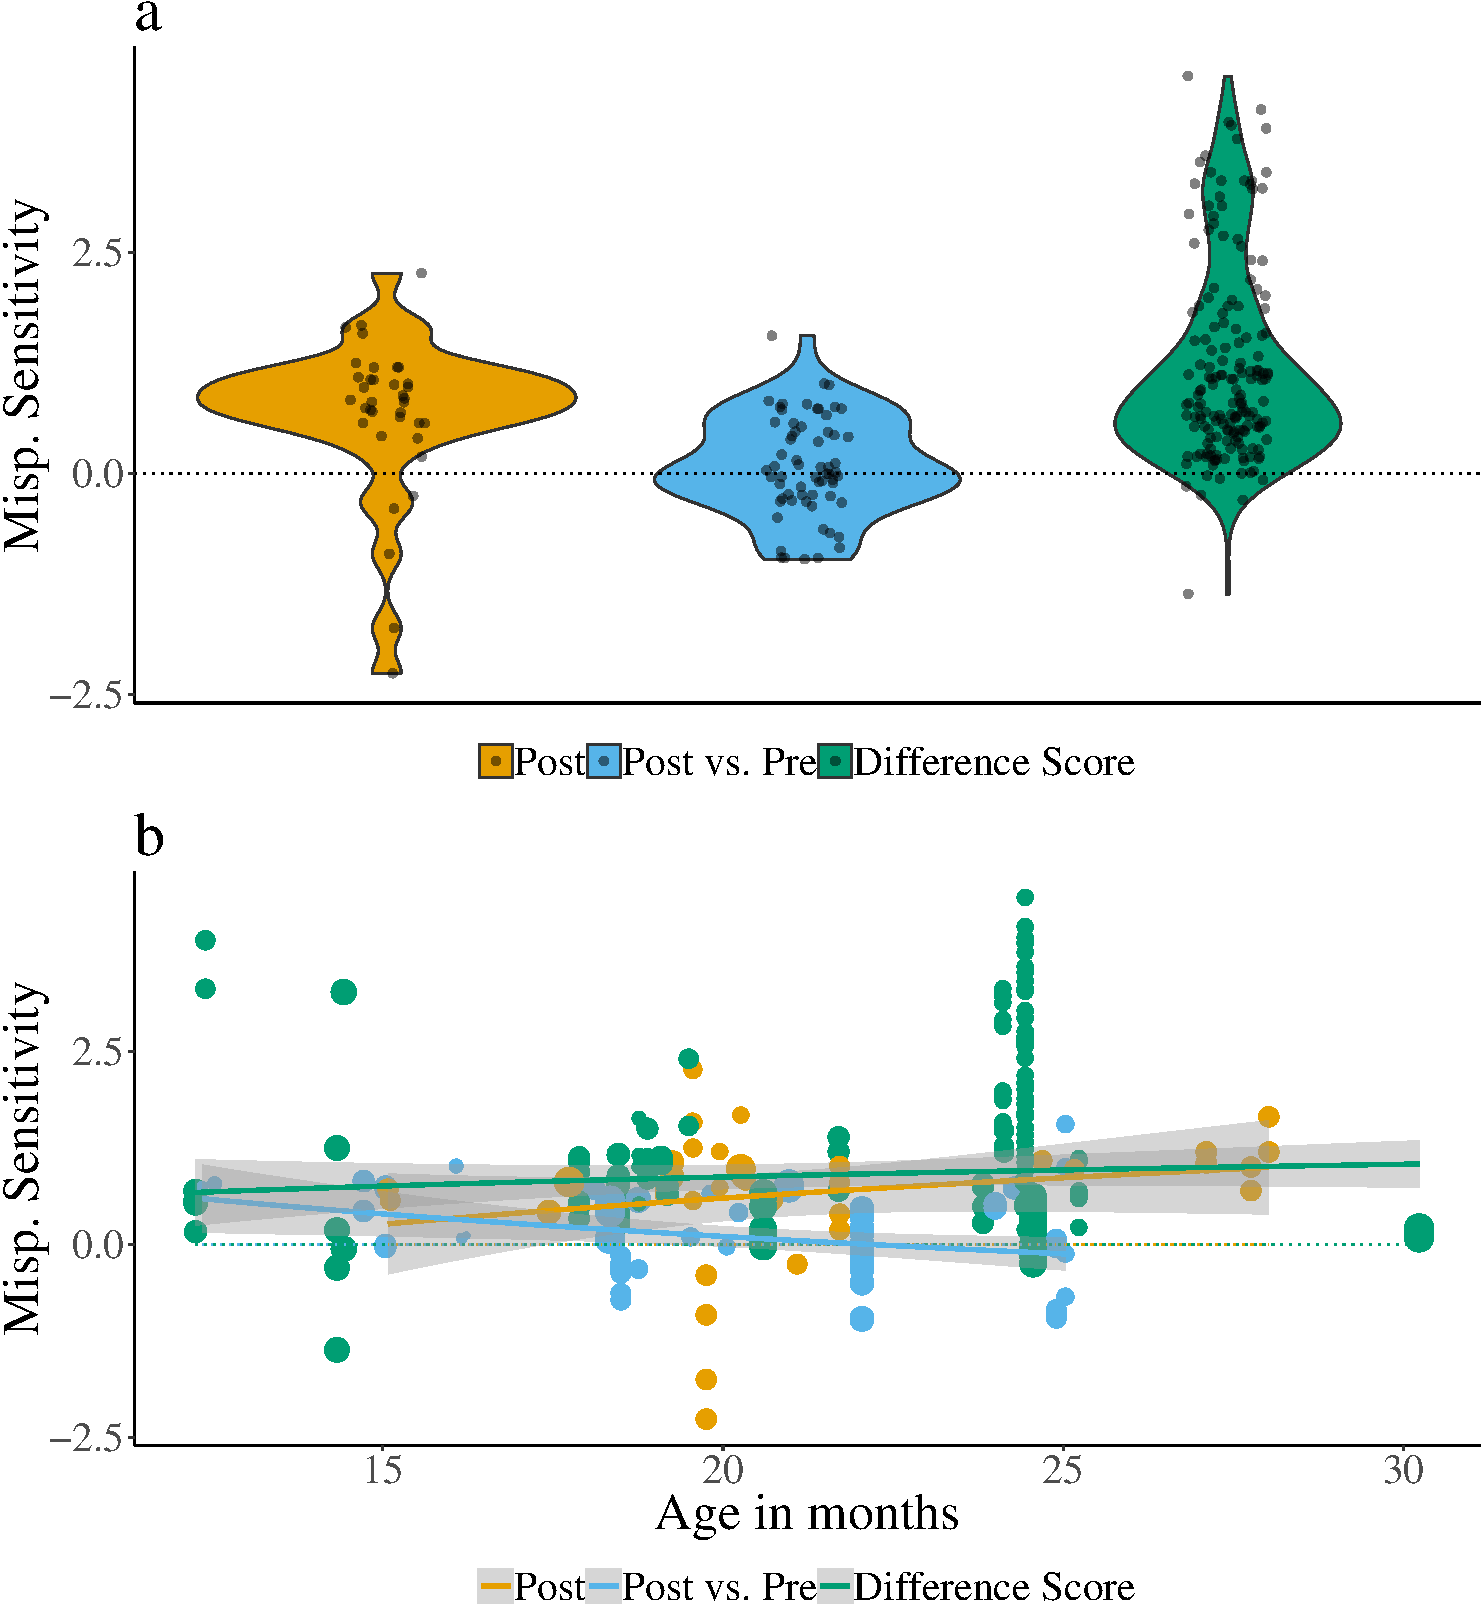
\includegraphics{Paper_Analyses_files/figure-latex/Plot_Within_cond_age_diff_score-1.pdf}
\caption{}
\end{figure}

\subsection{Controlling for researcher
choice}\label{controlling-for-researcher-choice}

\section{Discussion}\label{discussion}

To Summarize:

** Overall Meta-analytic Effect **

\begin{itemize}
\tightlist
\item
  Accept mispronunciations as labels for targets
\item
  Sensitive to mispronunciations
\item
  lack of change over development
\end{itemize}

** Vocabulary **

\begin{itemize}
\tightlist
\item
  no relationship?
\item
  talk about how few studies report it
\end{itemize}

** Data Analysis Choices **

\begin{itemize}
\tightlist
\item
  Post-naming phase size and dependent variable impact misp sensitivity
  development
\item
  Offset time does not impact misp sensitivity development
\item
  the first two do not have theoretical frameworks to guide researchers,
  whereas offset time does
\end{itemize}

When it comes to designing studies, best practices and current standards
might not always overlap. Indeed, across a set of previous meta-analyses
it was shown that particularly infant research does not adjust sample
sizes according to the effect in question (Bergmann et al., in press). A
meta-analysis is a first step in improving experiment planning by
measuring the underlying effect and its variance, which is directly
related to the sample needed to achieve satisfactory power in the null
hypothesis significance testing framework. Failing to take effect sizes
into account can both yield to underpowered research and to testing too
many participants, both consequences are undesirable for a number of
reasons that have been discussed in depth elsewhere. We will just
briefly mention two that we consider most salient for theory building:
Underpowered studies will lead to false negatives more frequently than
expected, which in turn results in an unpublished body of literature
(citationcitation). Overpowered studies mean that participants were
tested unnecessarily, which has substantial ethical consequences
particularly when working with infants and other difficult to recruit
and test populations.

From Christina: let's make a note to put sth in the discussion about our
curve being surprisingly flat for correctly pronounced words bc people
adapt their analysis windows? Bc if you look at Molly's reaction time
paper, there is a steep increase.

\newpage

\section{References}\label{references}

\begingroup
\setlength{\parindent}{-0.5in} \setlength{\leftskip}{0.5in}

\hypertarget{refs}{}

\endgroup


\end{document}
